\section{Group attention mechanism}
\label{sec.group}

\begin{sloppypar}
Group attention, a novel and efficient approximate attention mechanism, addresses the performance bottleneck of self-attention in the vanilla Transformer.
In this section, we first introduce the framework of group attention and then theoretically establish the bound of its approximation error.

\subsection{The Idea of Group Attention}
\label{sec.group.ideas}

As periodicity is a natural property of timeseries~\cite{10.1145/3448016.3452779}, similar windows frequently occur. Similar windows result in similar queries/keys for attention computation, bringing opportunities for saving computation.

% $O$ is calculated by:
% \begin{equation}
% \label{eq.selfattn}
% \begin{aligned}
% &a_{i,j}=\mathbf{q}_i \cdot \mathbf{k}_j \\
% &A_{i,j}=\frac{exp(a_{i,j})}{\sum_{k=0}^{n-1} exp(a_{i,k})}\\
% &\mathbf{o}_i=\sum_{j=0}^{n-1} A_{i,j}\mathbf{v}_j 
% \end{aligned}
% \end{equation}

%The content below is based on \eqref{eq.selfattn}.
As discussed in Sec.~\ref{sec.preliminary}, $A_{ij}$, the attention score of window $i$ onto window $j$, is determined by the inner product between the query vector of window $i$ and the key vector of window $j$, that is, $q_i \cdot k_j$. 
Given another window $x$, if window $x$ has the similar key vector to window $j$, that is, $k_j$ $\approx$ $k_x$, then $q_i \cdot k_j$ $\approx$ $q_i \cdot k_x$.
In other words, $A_{ij}$ $\approx$ $A_{ix}$ when $k_j$ $\approx$ $k_x$.

% %\textcolor{red}{formally. put fig 3}
% This observation inspires our group attention mechanism. That is, we group similar 
% keys and share attention computation in between. 
% To approximately represent the attention scores for keys in a group, we compute the attention score with {\it only one representative key}, for example, the center centroid of the group of keys.
% This thus saves significant computation cost.

This observation inspires our group attention mechanism. That is, we group the windows by their similarity in keys. 
Assuming all windows in the same group have the same attention score onto another window $k$, we then only compute the attention once by using {\it one single key} to represent this group, for example the centroid of the group of keys.
This thus saves significant computation cost.

Better yet, after grouping $n$ windows into $N$ groups, group attention compresses the attention matrix from an $n \times n$ matrix to an $n \times N$ matrix. Because $N$ (number of groups) tends to be much smaller than $n$ (number of windows) due to the periodicity of timeseries, group attention consumes much less memory than the original self-attention mechanism, successfully eliminating the memory bottleneck.  Note that it also doesn't hurt quality all that much, as confirmed in our experiments (Sec.~\ref{sec.exp.effective}).

% Denote $S_i$ to be the $i^{th}$ group, $COUNT_i$ to be the size of the $i^{th}$ group, $N$ to be the number of groups, $\mathbf{r}_i$ to be the representative key for the $i^{th}$ group and $\mathbf{R}$ to be the matrix consists of all $\mathbf{r}_i$, $BELONG_i$ to be the belonging group of $\mathbf{k}_i$, $\widetilde{\mathbf{k}}_i$ to be the representation of $\mathbf{k}_i$. 

% The grouping algorithm guarantees:
% $$S_i \cap S_j = \varnothing (i \neq j)$$
% $$\cup_{i=0}^{N-1} S_i= \cup_{i=0}^{n-1} \{\mathbf{k}_i\}$$

% Then, let
% $$\widetilde{\mathbf{k}}_{x}=\mathbf{r}_i$$

% such that
% $$\mathbf{k}_{x} \in S_i$$

% Output $\mathbf{o}$ of Group attention is calculated by
% \begin{equation}
% \label{eq.grpattn1}
% \widetilde{a}_{i,j}=\mathbf{q}_i \cdot \mathbf{\widetilde{k}_j} 
% \end{equation}

% \begin{equation}
% \label{eq.grpattn2}
% \widetilde{A}_{i,j}=\frac{exp(\widetilde{a}_{i,j})}{\sum_{k=0}^{n-1}exp(\widetilde{a}_{i,k})}
% \end{equation}

% \begin{equation}
% \label{eq.grpattn3}
% \widetilde{\mathbf{o}}_i=\sum_{j=0}^{n-1}\widetilde{A}_{i,j}\mathbf{v}_j
% \end{equation}

% As for all \textbf{keys} in the same group, the calculation of \eqref{eq.grpattn1} \eqref{eq.grpattn2} is the same, the calculation and storage is duplicate, bringing opportunity of optimization in performance. 

\begin{figure}[]
\vspace{-3mm}
    \centering    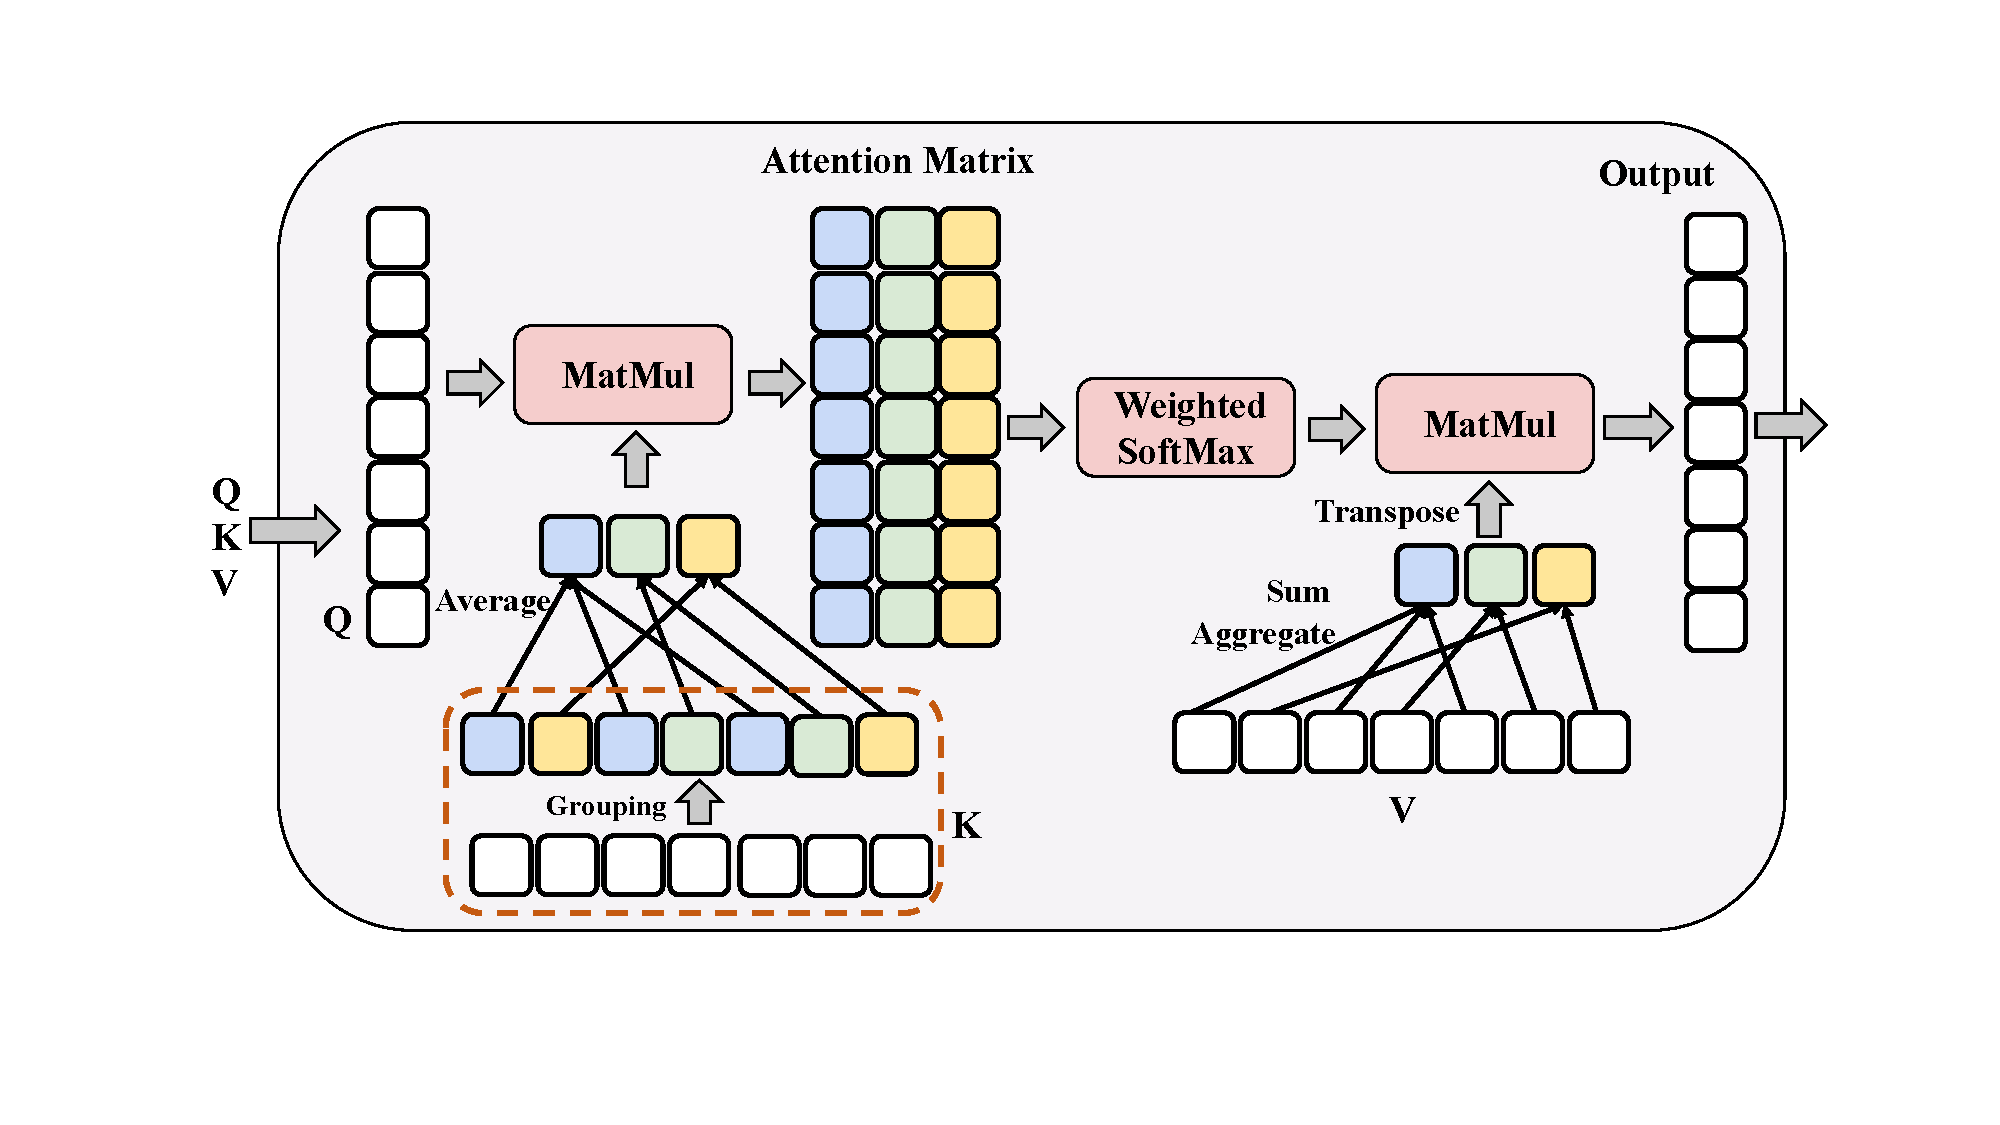
\includegraphics[width=1.05\columnwidth]{figures/attention.pdf}
    \vspace{-7mm}
    \caption{Group Attention}
    \label{fig.group}
    \vspace{-5mm}
\end{figure}

\subsection{Computing the Output Feature Embedding}
\label{sec.group.embedding}
We now discuss how to efficiently compute the output feature embeddings using the small compressed group attention matrix.

\vspace{-1mm}
\subsubsection{Problem: Producing Embeddings w/ Group Attention Matrix\nopunct}\ \\
As described in the Background, once we have acquired the attention matrix $A$, canonical self-attention computes the output embedding $O$ as $\mathit{O = AV}$. Because $A$ is an $n \times n$ matrix and $V$ is an $n \times d_v$ matrix, the matrix product operation still produces an $n \times d_v$ matrix $O$. That is, it produces a $d_v$ dimensional feature vector for each {\it window}.
However, our group attention will produce an $n \times N$ attention matrix $\widetilde{A}$ , where $N$ corresponds to the number of groups. 
In this case the matrix product will produce a $N \times d_v$ matrix $\widetilde{O}$. That is, it produces a feature vector for each {\it group}. 
However, our goal is to produce different embeddings for different windows, because even if some windows share the attention score temporally, it does not mean they should have the same feature embedding. 

%\jm{Accurately, restore P from $\widetilde{P}$. In GroupSoftmax, we say restore P from $\widetilde{P}$.}
\noindent\textbf{A Naive Solution.} A naive solution would be to restore the full attention matrix $A$ from the group attention matrix $\widetilde{A}$. For example, given one group composed of $win_i$ and $win_j$, we map its group attention vector in  $\widetilde{A}$ into two rows that correspond to $win_i$ and $win_j$ in $A$. 
However, in this case we again get a $n \times n$ attention matrix; and GPU memory remains a {\it bottleneck} in group attention.

\vspace{-1mm}
\subsubsection{Solution: Embedding Aggregation and Group SoftMax\nopunct}\ \\
\label{sec.group.efficient}
Using an \textit{embedding aggregation} operation and a \textit{group softmax} function, \system produces $n$ embeddings without restoring the full attention matrix. Fig.~\ref{fig.group} shows the workflow of group attention. 

\noindent\textbf{Embedding Aggregation.} The idea is inspired by the observation on the matrix product operation $\mathit{O = AV}$ conducted on the fully restored attention matrix $A$. 

Given an element $O_{i,j}$ of $O$ corresponding to the $j^{th}$ dimension of $win_i$'s feature vector, $O_{i,j}$ = $a_i \cdot v_j$, where vector $\mathit{a_i \in \mathbb{R}^{n}}$ denotes the $i^{th}$ row of the attention matrix $A$ and vector $\mathit{v_j \in \mathbb{R}^{n}}$ denotes the $j^{th}$ dimension of all the $n$ feature vectors. 
Given $\mathit{a_i = <a_i^1, a_i^2, \cdots, a_i^n>}$ and $\mathit{v_j = <v_j^1, v_j^2, \cdots, v_j^n>}$, $O_{i,j}$ = $\mathit{\sum_{k=1}^n a_i^k v_j^k}$.
%$(i=1,...,n,j= 1,...,d_v)$

As an example, assume $win_1$ and $win_2$ belong to the same group $G_1$. Then $a_i^1$ = $a_i^2$ = $\widetilde{a}_i^1$, where $\widetilde{a}_i^1$ $\in$ $\widetilde{A}$ corresponds to the attention of group $G_1$ onto $win_i$. 
Therefore, $a_i^1 v_j^1$ + $a_i^2 v_j^2$ = $\widetilde{a}_i^1$ ($v_j^1$ + $v_j^2$).

As an immediate generalization of the above analysis, if we aggregate up the windows that belong to the same group and convert the n-dimensional feature vector $v_j$ into a $N$-dimensional group feature vector $\widetilde{v}_j$ beforehand, we could directly use the group attention vector $\widetilde{a}_i$ and the group feature vector $\widetilde{v}_j$ to compute $O_{i,j}$.

Using embedding aggregation, \system is able to produce the feature embedding $\widetilde{O}$ that is identical to the embedding $O$ produced by using the full attention matrix $A$ and the embedding matrix $V$.

\noindent\textbf{Group Softmax Function.}
In canonical self-attention the attention matrix $A$ is computed as $A$ = $\mathit{SoftMax(\frac{QK^T}{\sqrt{d_k}})}$. To compute $A$, we have to first compute $QK^T$ (denoted as $P$) which is an $n \times n$ matrix. Then normalizing the $P$ matrix with softmax produces the attention matrix $A$. 

Group attention follows the same procedure. But after grouping keys into $\widetilde{K}$, $Q\widetilde{K}^T$ produces an $n \times N$ matrix $\widetilde{P}$. Due to the non-linearity of the softmax function, applying softmax directly on $\widetilde{P}$ will result in a group attention matrix $\widetilde{A}$ from which we are not able to recover a full attention matrix that is identical to first restoring $\widetilde{P}$ to $P$ and then applying softmax on $P$. The $A$ matrix produced by the latter is desirable, as we want to approximate the original attention matrix as accurately as possible. 
However, restoring the small $n \times N$ $\widetilde{P}$ matrix is not memory efficient, as it will end up with a full $n \times n$ matrix $P$. %This is exactly what group attention tries to avoid. 

To solve the above problems, we introduce a new \textbf{group softmax} function to replace the original softmax function (Eq.~\ref{eq.softmax}).

\vspace{-2mm}
\begin{equation}
\label{eq.groupSoftmax}
GroupSoftMax(\widetilde{P_{i,j}}) = \frac{exp(P_{i,j})}{\sum_{k=0}^{N-1} count_k exp(P_{i,k})}\\
\end{equation}

In Eq.~\ref{eq.groupSoftmax}, $count_k$ represents the number of windows that Group $G_k$ contains. Compared to the original softmax, our group softmax considers each group $G_k$ as $count_k$ elements and counts it $count_k$ times when summing up the exponential of each group's $P_{i,k}$.
In this way, the group softmax function operating on the small $\widetilde{P}$ matrix will produce {\it exactly the same} result to the softmax function operating on the full $P$ matrix.

\noindent\textbf{Theoretical Guarantee.} In Appendix~\ref{appendix.proof.groupAttention}, we prove that the group softmax function and the embedding aggregation operation produce the same output feature embedding with the naive method that has to first restore the big full attention matrix.

We show an efficient implementation of the embedding aggregation operation and group softmax function in Appendix~\ref{appendix.groupAttention}, Alg.~\ref{algo.grpattn}.

\noindent\textbf{Time Complexity.}
%, and $\widetilde{\mathbf{k}}_i$ to be the representation of $\mathbf{k}_i$
%of which the time complexity is $O(nNd)$ and the space complexity is $O(nN)$.
The time complexity of Alg.~\ref{algo.grpattn} is $O(nNd)$ and the space complexity is $O(nN)$, while the time and space complexity of the original self-attention mechanism are $O(n^2d)$ and $O(n^2)$.

 

\begin{comment}
\subsubsection{Correctness Proof of Group attention\nopunct}\ \\
\label{sec.group.correctness}
\vspace{-2mm}
In this section, we prove that the group softmax function as well as the embedding aggregation operation produce the same output feature embedding with the naive method that has to first restore the big full attention matrix. 
Note in group attention's computation, we use a representative vector to represent all the key vectors in the $i^{th}$ group, thus satisfying the assumption made in Lemma~\ref{lm.grpattnalgo}. 

\begin{lemma}
\label{lm.grpattnalgo}
\sloppypar
Assuming the windows belonging to the same group $G_i$ have the same key vector, i.e. $k_j=r_i (win_j \in G_i)$, then the feature embedding $O$ produced by the original self-attention mechanism is identical to the output of our group attention mechanism implemented in Algorithm~\ref{algo.grpattn}.

%outputs the same \textbf{o} with \eqref{eq.grpattn1} \eqref{eq.grpattn2} \eqref{eq.grpattn3}.
\end{lemma}

Due to space limits, please refer to our technical report~\cite{RITA} for the proof.


\begin{proof}
Denote $\widetilde{k_j}$ to be the representative vectors of $k_j$, i.e. $\widetilde{k_j}=r_i=k_j (win_j \in G_i)$. Algorithm~\ref{algo.grpattn} gives that
\begin{equation}
\label{eq.grpres}
\begin{aligned}
    \widetilde{v}_i&=\sum_{j=0}^{n-1}(BELONG_j==i)\mathbf{v}_j, \ \widetilde{P}_{i,j}&=\mathbf{q}_i \cdot \mathbf{r}_j\\
    s_i&=\sum_{j=0}^{N-1}exp(\widetilde{P}_{i,j})COUNT_j, \ \widetilde{o}_i&=\sum_{j=0}^{N-1}\frac{\widetilde{P}_{i,j}}{s_i}\widetilde{v}_j
\end{aligned}
\end{equation}

By the classical self-attention mechanism introduced in Sec.~\ref{sec.preliminary.transformer}, we get:
\begin{equation}
\label{eq.grpattn1}
P_{i,j}=\mathbf{q}_i \cdot \mathbf{k_j},\ A_{i,j}=\frac{exp(P_{i,j})}{\sum_{k=0}^{n-1}exp(P_{i,k})}, \ \mathbf{o}_i=\sum_{j=0}^{n-1}A_{i,j}\mathbf{v}_j
\end{equation}

% \begin{equation}
% \label{eq.grpattn2}
% A_{i,j}=\frac{exp(P_{i,j})}{\sum_{k=0}^{n-1}exp(P_{i,k})}
% \end{equation}

% \begin{equation}
% \label{eq.grpattn3}
% \mathbf{o}_i=\sum_{j=0}^{n-1}A_{i,j}\mathbf{v}_j
% \end{equation}

With \ref{eq.grpres} and \ref{eq.grpattn1}, we have
\begin{equation}
\label{eq.sumexpahat}
\begin{aligned}
    \sum_{j=0}^{n-1}exp(P_{i,j})&=\sum_{j=0}^{n-1}exp(\mathbf{q}_i \cdot \mathbf{k}_j)\\
    &=\sum_{j=0}^{N-1} \sum_{x=0}^{n-1}(BELONG_x==j)exp(\mathbf{q}_i \cdot \mathbf{k}_x)\\
    &=\sum_{j=0}^{N-1} exp(\mathbf{q}_i \cdot \mathbf{r}_j) \sum_{x=0}^{n-1} (BELONG_x==j) \\
    &=\sum_{j=0}^{N-1} exp(\mathbf{q}_i \cdot \mathbf{r}_j) COUNT_j
    \\
    &=\sum_{j=0}^{N-1} exp(\widetilde{P}_{i,j}) COUNT_j\\
    &=s_i\\
\end{aligned}
\end{equation}


Further,

\begin{equation}
\label{eq.output}
\begin{aligned}
\mathbf{o}_i&=\sum_{j=0}^{n-1} A_{i,j}\mathbf{v_j} \\
&=\sum_{j=0}^{N-1}\sum_{x=0}^{n-1} (BELONG_x==j)A_{i,x}\mathbf{v}_x \\
&=\sum_{j=0}^{N-1}\sum_{x=0}^{n-1}(BELONG_x==j)\frac{exp(P_{i,x})}{\sum_{k=0}^{n-1}exp(P_{i,k})}\mathbf{v}_x\\
&=\sum_{j=0}^{N-1}\sum_{x=0}^{n-1}(BELONG_x==j)\frac{exp(\mathbf{q}_i \cdot \mathbf{k}_x)}{\sum_{k=0}^{n-1}exp(P_{i,k})}\mathbf{v}_x\\
&=\sum_{j=0}^{N-1}\sum_{x=0}^{n-1}(BELONG_x==j)\frac{exp(\mathbf{q}_i \cdot \mathbf{r_j})}{\sum_{k=0}^{n-1}exp(P_{i,k})}\mathbf{v}_x\\
&=\sum_{j=0}^{N-1} \frac{exp(\mathbf{q}_i \cdot \mathbf{r_j})}{\sum_{k=0}^{n-1}exp(P_{i,k})} \sum_{x=0}^{n-1}(BELONG_x==j)\mathbf{v}_x\\
&=\sum_{j=0}^{N-1} \frac{exp(\mathbf{q}_i \cdot \mathbf{r_j})}{\sum_{k=0}^{n-1}exp(P_{i,k})} \widetilde{v_j}\\
\end{aligned}
\end{equation}

Combining \eqref{eq.grpres}, \eqref{eq.sumexpahat} \eqref{eq.output}, we have
$\mathit{\mathbf{o}_i=\sum_{j=0}^{N-1}\frac{\widetilde{P}_{i,j}}{s_i}\widetilde{v}_j=\widetilde{o}_i}$.

This concludes that the output of our group attention is identical to vanilla self-attention's.
\end{proof}
\end{comment}

\subsection{Error Bound}
\label{sec.group.error}

Group attention produces a group attention matrix $\widetilde{A}$ which approximates the attention matrix $A$ produced by the classical self-attention with a {\it bounded error}, as shown in Lemma~\ref{lm.grperrorbound}.
\vspace{-1mm}
\begin{lemma}
\label{lm.grperrorbound}
Let $R$ be the radius of the ball where all key vectors live; $\widetilde{k}_i$ be the representative of the group that contains key $k_i$. Let $\overline{A}$ denote the full attention matrix restored from $\widetilde{A}$. Suppose the distance between $\widetilde{k}_i$ and $k_i$ $(||\widetilde{\mathbf{k}}_i-\mathbf{k}_i||)$ satisfies: $||\widetilde{\mathbf{k}}_i-\mathbf{k}_i|| \leq$ {\bf d}.

Then $\forall$ $\epsilon > 1$, if $\mathit{d \leq \frac{\ln(\epsilon)}{2R}}$, $\mathit{\frac{1}{\epsilon} \leq \frac{\overline{A}_{i,j}}{A_{i,j}} \leq \epsilon}$
\end{lemma}

Lemma~\ref{lm.grperrorbound} shows that the error bound $\epsilon$ of the group attention is determined by the distance $d$. 
As discussed in Sec.~\ref{sec.scheduler.group}, it inspires us to design a strategy to dynamically determine the number of groups $N$ -- the most critical parameter of group attention. 
Please refer to Appendix~\ref{appendix.proof.errorBound} for the proof. 

\begin{comment}
\begin{proof}
We have
\begin{equation}
\begin{aligned}
    \frac{exp(\widetilde{P}_{i,j})}{exp(P_{i,j})}&=\frac{exp({\mathbf{q}}_i \cdot \widetilde{\mathbf{k}}_j)}{exp(\mathbf{q}_i \cdot \mathbf{k}_j)} = exp({\mathbf{q}}_i \cdot (\widetilde{ \mathbf{k}}_j-\mathbf{k}_j))\\
%   &= exp({\mathbf{q}}_i \cdot (\widetilde{ \mathbf{k}}_j-\mathbf{k}_j))\\
   &=exp(||\mathbf{q}_i||||\widetilde{\mathbf{k}}_j-\mathbf{k}_j||cos(\mathbf{q}_i,\widetilde{\mathbf{k}}_j-\mathbf{k}_j))
\end{aligned}
\end{equation}

So
\begin{equation}
\label{equ.abound}
exp(-dR) \leq \frac{exp(\widetilde{P}_{i,j})}{exp(P_{i,j})} \leq exp(dR)
\end{equation}

Then we have:
\begin{equation}
\label{equ.Aequ}
\begin{aligned}
\frac{\widetilde{A}_{i,j}}{A_{i,j}}&=\frac{exp(\widetilde{P}_{i,j})}{\sum_{k=1}^{n} exp(\widetilde{P}_{i,k})} / \frac{exp({P}_{i,j})}{\sum_{k=1}^{n} exp({P}_{i,k})}\\
&=\frac{exp(\widetilde{P}_{i,j})}{exp({P}_{i,j})} \frac{\sum_{k=1}^{n} exp({P}_{i,k})}{\sum_{k=1}^{n} exp(\widetilde{P}_{i,k})}
\end{aligned}
\end{equation}

Combining (\ref{equ.abound}) (\ref{equ.Aequ}), the error is bounded by
\begin{equation}
\label{equ.Abound}
exp(-2dR) \leq \frac{\widetilde{A}_{i,j}}{A_{i,j}} \leq exp(2dR)
\end{equation}

Thus, if $\mathit{d \leq \frac{\ln(\epsilon)}{2R}}$, $\mathit{\frac{1}{\epsilon} \leq \frac{\widetilde{A}_{i,j}}{A_{i,j}} \leq \epsilon}$. This proves Lemma~\ref{lm.grperrorbound}.
\end{proof}
\end{comment}


\subsection{GPU Friendly Grouping Method}
In this section, we discuss the implementation of a grouping method. To make group attention efficient and effective, the grouping method has to satisfy the following requirements: 

(1) Tight distance bound: to ensure the approximation quality, the distance between each key and its group representative should be minimized according to Lemma~\ref{lm.grperrorbound}.

(2) Lightweight: to ensure the performance gain, the grouping method must be lightweight, at worst not exceeding the complexity of group attention itself ($O(Nn)$).

(3) GPU friendly: to take advantage of GPUs, we prefer a grouping method that mainly consists of matrix operations, which can be efficiently executed on a GPU.

To satisfy the above requirements, after thorough investigation on various clustering algorithms, we design a GPU friendly K-means~\cite{lloyd1982least} as the grouping method. 

First, K-means minimizes the overall distance between any object and its cluster center, hence naturally satisfying Requirement 1. 

Second, given $N$ centers, in each iteration the time and space complexity of K-means is $O(nN)$. Usually, the iteration goes until convergence. However, we observe that rather than seeking a perfect K-means clustering, training a few iterations is sufficient to get a good grouping for group attention, because typically the later iterations only slightly update the clustering and group attention is robust to such imperfection. 

Third, we design a GPU-friendly implementation of K-means. The performance bottleneck of K-means comes from the distance computation between each vector and its center, that is, $\mathit{|v_i-c_j|=\sqrt{(v_i-c_j)^2}, i\in [1,n], j\in [1,N]}$. The performance bottleneck is $v_i-c_j$.
We instead use a different formulation: $|v_i-c_j|=\mathit{|v_i-c_j|=\sqrt{|v_i|^2+|c_j|^2-2 v_i \cdot c_j}, i\in [1,n], j\in [1,N]}$.
This is because in this formulation, the performance bottleneck is $v_i \cdot c_j$, which could be implemented as a matrix product operation.
Although the complexity of the two formulations is the same, in GPUs matrix product is much more efficient than pairwise difference.

% \noindent\textbf{Formalization}

% Given $n$ vectors $v_1,v_2,...,v_n \in \mathbf{R}^d$ and a threshold $d$. Determine the clusters, satisfying the Euclidean distance between two vectors $|v_i-v_j|<d$ if $v_i$ and $v_j$ are in a same cluster. 


% \noindent\textbf{Eculidean LSH}

% The hash bucket that vector $v$ falls into is given by:
% \begin{equation}
%     \label{eq.eculsh}
%     H(v)=\lfloor \frac{v \cdot x+b}{w} \rfloor
% \end{equation}
% Where $w\in \mathbf{R}$ is a hyper-parameter, $x\in \mathbf{R}^d$ is sampled from \emph{p-stable} distribution and $b \in \mathbf{R}$ is sampled uniformly from $[0,w]$.

% \cite{} shows that the probability $v_1,v_2$ getting to the same bucket is:
% \begin{equation}
%     \label{eq.lsh_prob}
%     P[H(v_1)=H(v_2)]=\int_0^w {\frac{1}{u} f(\frac{t}{u})(1-\frac{t}{w}) dt}
% \end{equation}

% Where $u=|v_1-v_2|$ and $f$ is the probability density function of the \emph{p-stable} distribution. 

% As for our implementation, we conduct Euclidean LSH, then drop the empty buckets and treat the remaining buckets as groups. One should notice that choosing a proper $w$ remains a problem and we will discuss that in experiments.\\
\end{sloppypar}